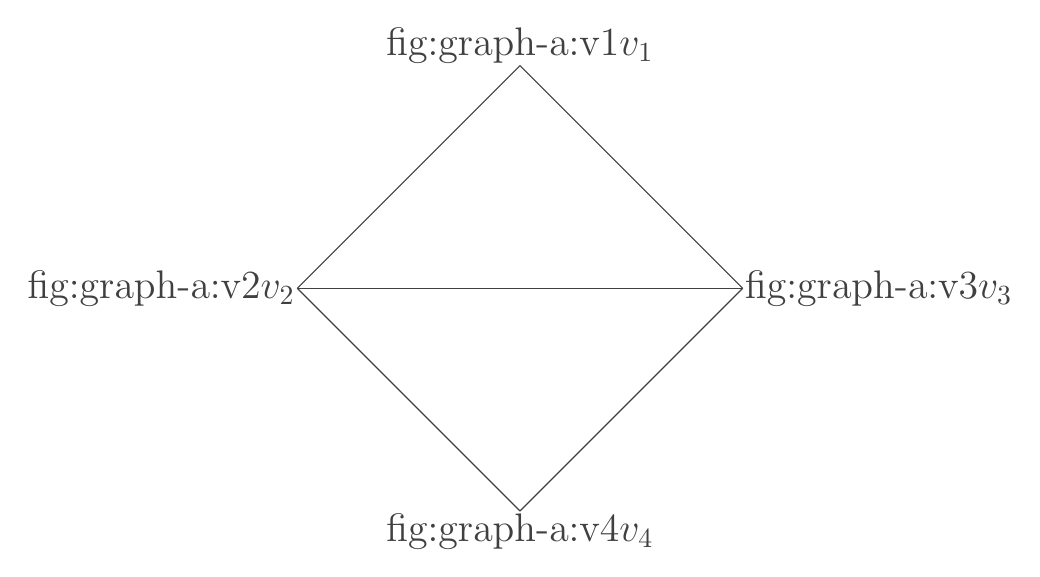
\begin{tikzpicture}[draw=darkgray, text=darkgray, align=center, node distance=4cm]
    \tikzstyle{every node}=[inner sep=0pt];

    \node (v1) [label=above:{\Large\hypertarget{fig:graph-a:v1}{$v_1$}}] {};
    \node (v2) [label=left:{\Large\hypertarget{fig:graph-a:v2}{$v_2$}}, below left of = v1] {};
    \node (v3) [label=right:{\Large\hypertarget{fig:graph-a:v3}{$v_3$}}, below right of = v1] {};
    \node (v4) [label=below:{\Large\hypertarget{fig:graph-a:v4}{$v_4$}}, below right of = v2] {};

    \path (v1.center)
        edge (v2.center)
        edge (v3.center);
    \path (v4.center)
        edge (v2.center)
        edge (v3.center);
    \path (v2.center)
        edge (v3.center);
\end{tikzpicture}
